\chapter{Alg : Algebraic Functional Language} \label{chap:alg}
Algebraic Functional Language (Alg) is an example of a high-level language to generate parallel code, proposed in the paper \cite{AlgebraicMultipartyProtocol}. The work done by \cite{AlgebraicMultipartyProtocol} also proposes a method to do the code generation. Part of this project is about implementing an alternative code generation backend for this language. In the evaluation section, we will compare the speed of the generated code of our method against the original method. We will give an overview of the language in this section.  
\section{Alg}
\subsection{Syntax}
\begin{table}[ht]
\begin{grammar}{F_1, F_2 \Coloneqq}{}
    I & Identity functor\\
    K t & Constant functor\\
    F_1 + F_2 & Sum functor\\
    F_1 \times F_2 & Product functor
\end{grammar}
\hfill
\begin{grammar}{t_1, t_2 \Coloneqq}{Type}
    () \mid \text{int} \mid \dots & Primitive types\\
    a \rightarrow b & Function types\\
    a + b & Sum types \\
    a \times b & Product types\\
    F \ t_1 & Functor types\\
    \mu .F & Recursive types\\
\end{grammar}
\vskip\baselineskip
\begin{grammar}{e_1, e_2 \Coloneqq}{Expression}
    f \mid v \mid \text{const $e$} \mid e_1 \circ e_2 \mid \pi_i \mid e_1 \vartriangle e_2 \mid e_1 \triangledown e_2 \mid l_i \mid F \; e \mid \text{in}_F \mid \text{out}_F \mid \text{rec}_F \; e_1 \; e_2
\end{grammar}
\caption{Syntax of Alg language}
\label{project:syntax}
\end{table}
\begin{listing}[ht]
\begin{lstlisting}{language=Haskell}
    newtype L = K () + K Int * I
    type List = Rec L
\end{lstlisting}
\caption{Type of integer list in PAL}
\label{p:pal:c1}
\end{listing}
The syntax of Alg is shown in \tabref{project:syntax}. In terms of the syntax of expressions, $f$ represents atomic functions which are functions of which we only know their types \cite{AlgebraicMultipartyProtocol}. The presence of atomic functions is important in the code generation, which we will discuss in the later chapter. $v$ is a primitive value like integer 1.$F$ represents functor and $a, b$ are types. Besides primitive types, function types and the recursive type constructor $\mu$, Alg uses four functors to form more types hence representing data structures by composing them. For example, a list of integers is expressed in \coref{p:pal:c1}. Alg is a point-free language.
\begin{table}[ht]
    \[\inference{f : a -> b \in \Gamma}{|- f : a -> b}\]
    \[\inference{|- e : a}{|- \text{cons} \; e : b -> a}\]
    \[\inference{}{|- \text{id} : a -> a}\]
    \[\inference{}{|- \text{in}_F : F \; \mu F -> \mu F}\]
    \[\inference{}{|- \text{out}_F : \mu F -> F \; \mu F}\]
    \[\inference{|- e_1 : b -> c, \quad |- e_2 : a -> b}{e_1 \circ e_2: a -> b}\]
    \[\inference{i \in [1,2]}{\pi_i : a_1 \times a_2 -> a_i}\]
    \[\inference{i \in [1,2]}{l_i : a_i -> a_1 + a_2}\]
    \[\inference{|- e_1 : a -> b, \quad |- e_2 : a -> b}{e_1 \vartriangle e_2: a -> b \times c}\]
    \[\inference{|- e_1 : a -> c, \quad |- e_2 : b -> c}{e_1 \triangledown e_2: a + b -> c}\]
    \[\inference{|- e : a -> b}{F \; e : F \; a -> F \; b}\]
    \[\inference{|- e_1 : F \; b -> b, \quad |- e_2 : a -> F \; a}{\text{rec}_F \; e_1 \; e_2: a -> b}\]
    \caption{Typing rules for Alg}
    \label{project:typing}
\end{table}
\begin{table}[ht]
    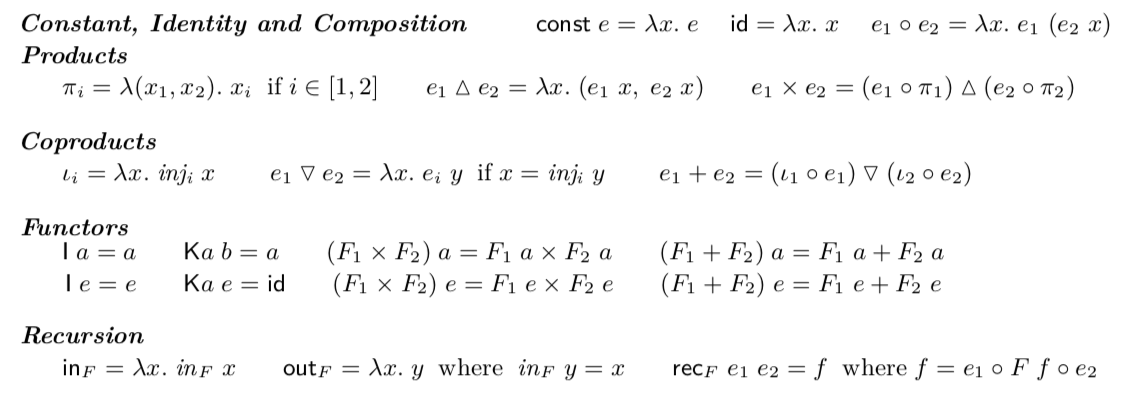
\includegraphics[width=\textwidth]{project/semantics.png}
    \caption{Semantics of Alg expression\cite{AlgebraicMultipartyProtocol}} 
    \label{project:Semantics}
\end{table}

The typing rules for Alg are expressed in \tabref{project:typing} and the semantics for Al is shown in \tabref{project:Semantics}. 

An important feature of Alg is the lack of usual control flow like if a branch or while loop to build algorithms, instead, it uses the flow of transformation of data structures to replace conventional control flow. For example, $\triangledown$ combinator is the case operation whose types is $a + b \rightarrow c$. It can be seen as an analogy of if branch in normal programming languages. $\vartriangle$ combinator represents split operation. More importantly, the combinator $\text{rec}_F$ uses the idea of recursion schemes (explained in \secref{b:rs}) to build divide-and-conquer algorithms. 

To summarize, algorithms in Alg are represented as a series of transformations of data, making it easy to transform the Alg programs to programs in arrows mechanically since arrows also express the flow of data and their transformations naturally. This property allows us to generate parallel code without burdens.

\begin{listing}[ht]
\begin{align*}
\mathbf{ms} &= \text{rec}_T \; \text{mrg} \; \text{spl} = \text{mrg} \circ T \; (\text{rec}_T \; \text{mrg} \; \text{spl}) \circ \text{spl} \\
& = \text{mrg} \circ (\text{id} + \text{id} + (\text{rec}_T \; \text{mrg} \; \text{spl}) \times (\text{rec}_T \; \text{mrg} \; \text{spl})) \circ \text{spl} \\
& = \text{mrg}  \circ (\text{id} + \text{id} + \mathbf{ms} \times \mathbf{ms}) \circ \text{spl}
\end{align*}
\caption{Merge sort in Alg} \label{p:pal:c5}
\end{listing}

By making the hylomorphism as a built-in combinator $\text{rec}_F$, Alg can express merge sort similarly as the example shown in \secref{b:rs:ex}. We use the functor $T = K () + K a + I \times I $ to be substitute the functor $F$ in $rec_F$ and the type $Ls$ to represent a list of elements whose type is $a$. We also have two atomic function spl : $Ls \rightarrow T \; Ls$ and mrg : $T \; Ls \rightarrow Ls$. Finally we express merge sort as $\mathbf{ms} = \text{rec}_T \; \text{mrg} \; \text{spl}$. It is shown in \coref{p:pal:c5}. From the example, we observe that $\mathbf{ms}$ can expanded infinitely. Later, we will exploit this property to generate parallel code. 

\section{ParAlg: Alg + role annotations}
% Each of the Alg constructs has an implicit, but precise data-flow. For example, in e1 ◦ e2, we know that the result of e1 must only use the result of e2. In a sense, we can interpret that e2, and only e2 sends a message to e1. In this section, we extend this interpretation to most of Alg constructs, so that Alg expressions represent both functions and protocols. We call this extension Parallel Algebraic Language (ParAlg). We define first the syntax of ParAlg terms and types, which is a subset of that of Alg that introduces role annotations that represent where is the computation performed and the data stored. We then define a typing derivation for ParAlg that captures the role interfaces of a ParAlg expression. In §4, we prove that well-typed Parallel Algebraic Language expressions, i.e. expressions built by composing sub-expressions that agree on their role interfaces, exactly correspond to deadlock-free global types (Lemmas 4.5 and 4.6).
Alg programs are point-free programs which have an implicit but precise data-flow that does not rely on an external context. For example, $e_1 \circ e_2$ is the function composition so the output of applying $e_2$ will be used as the input of $e_1$. We can interpret this as $e_2$ sends a message to $e_1$. Parallel Algebraic Language is the formalization of the above idea. In essence, it is Alg with role annotations, converting implicit data-flow to explicit role communication. In this section, we will present the main results and use examples to build intuitions about its principles. More details and proofs can be found in \cite{AlgebraicMultipartyProtocol}. We will briefly mention the results that will be useful in our project.

\subsection{Syntax}
\begin{table}[ht]
    \centering
    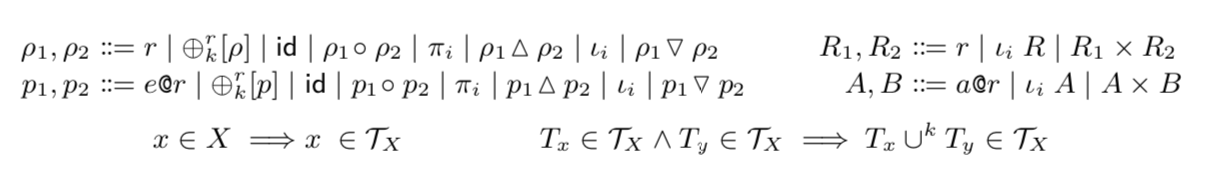
\includegraphics[width=\textwidth]{project/paralg.png}
    \caption{Syntax of ParAlg}
    \label{project:tab:paralg}
\end{table}
The syntax of ParAlg is shown in \tabref{project:tab:paralg}. $r$ is the role identifier representing a unit of computation. $R_1 \times R_2$ specifies that the input is split across roles $R_1$ and $R_2$ \cite{AlgebraicMultipartyProtocol}. More explanation of different constructor can be seen in \cite{AlgebraicMultipartyProtocol}. In short, ParAlg is just Alg with role annotations at certain points. 

Notice that $\text{rec}_F$ in Alg does not belong to constructs of ParAlg. So we need to unroll recursion a fixed number of times and then apply the role annotations to the unrolled expression. The unroll process is shown in \coref{p:pal:c5} and in this example, the number of unrollings is 1. The unroll-and-annotate operation will parallelize the recursive functions.
\subsection{Inferring global types}
ParAlg turns implicit data-flow into communication, and hence, we should be able to derive its communication protocols from valid ParAlg programs. In \cite{AlgebraicMultipartyProtocol}, global types (explained in \secref{b:mpst}) are used to represent communication protocols for ParAlg, which means for any valid ParAlg program, we can infer its corresponding global type. The inference rules and typing for ParAlg can be seen in \cite{AlgebraicMultipartyProtocol}. 
\begin{listing}[ht]
    \begin{align*}
       G = \\ 
       & r_0 -> r_1: \text{Rec L} \\
       & r_1 -> \{r_2, r_3\}\\
       & \{ l_0 : r_1 -> r_3 : () + \text{int}.\\
       & \quad \text{end};\\
       &  l_1 :  r_1 -> r_2 : \text{Rec L}.\\
       &  \,\quad  r_1 -> r_3 : \text{Rec L}.\\
       &  \,\quad  r_2 -> r_3 : \text{Rec L}.\\
       &  \,\quad  \text{end} \}; \\
       & r_3 -> r_0 : \text{Rec L}.\\
       & \text{end}\\
    \end{align*}
    \caption{Global types for merge sort}
    \label{project:code:ms2}
\end{listing}

An example of the inferred global type is in \coref{project:code:ms2}. It is the inferred global type of $\text{rec}_T$ mrg spl with the number of unrollings equal to two. This global type tells us that $r_1$ receives an input list from $r_0$, based on the length of the input list, $r_1$ either sends it to $r_3$ directly when the list is a singleton or empty or splits the list into halves and sends them to $r_2$ and $r_3$ respectively. In the second case, $r_2$ processes the received list and sends it to $r_3$, $r_3$ processes its received part and waits for another half of list to be received from $r_2$. After both $r_2$ and $r_3$ finish, $r_3$ will process the combined results. Finally $r_3$ sends the data back to $r_0$.

\subsection{Example: Parallel merge sort}
\begin{listing}[ht]
\inputminted{text}{project/ms.txt}
\caption{ParAlg for merge sort}
\label{project:code:mspar}
\end{listing}

The ParAlg expression for two unrolling of the merge sort is shown in \coref{project:code:mspar}. We use arrow combinators \hask{&&&} and \hask{|||} to replace $\triangledown$ and $\vartriangle$ in the actual ParAlg expression since they are equivalent. A similar reason also applies to \hask{inj}, the replacement of $l_i$ and \hask{proj}, the replacement of $\pi_i$. Its inferred global type is shown in the last subsection.

\section{Conclusion}
\begin{figure}[ht]
    \centering
    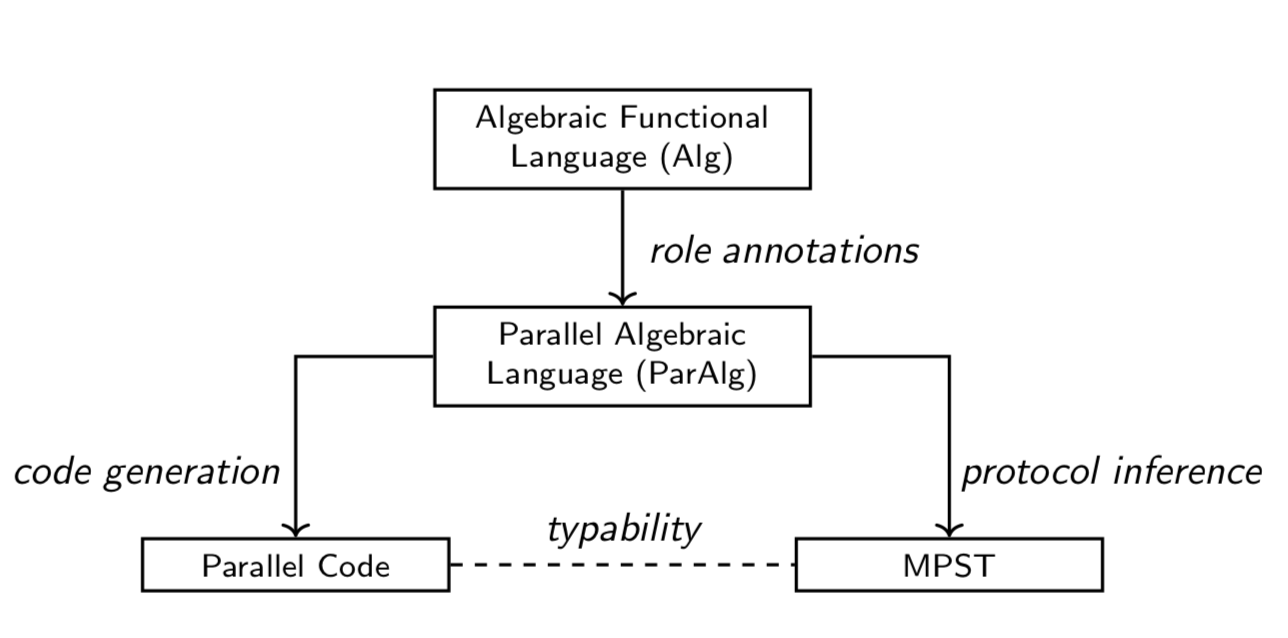
\includegraphics[width=0.7\textwidth]{project/pipeline.png}
    \caption{Overview of code generating pipeline from Alg\cite{AlgebraicMultipartyProtocol}}
    \label{project:fig:pipeline}
\end{figure}
A visualization of the compilation pipeline can be seen in the \figref{project:fig:pipeline}. More details about Alg and ParAlg can found in \cite{AlgebraicMultipartyProtocol}.

Alg is a point-free language. Without the use of explicit variables, point-free programs express the underlying data-flow of the computation clearly. Adding role annotations transforms Alg programs to ParAlg programs converting the implicit data-flow to explicit communication. Communication will aid us to generate parallel code using message-passing concurrency. We will introduce our method from the next chapter.